\documentclass{beamer}
\usepackage[utf8]{inputenc}
\usepackage{helvet}
\usepackage[spanish]{babel}
\usepackage{tikz}
\usetikzlibrary{shapes.multipart}
\usetikzlibrary{arrows,shapes,trees}
\usetikzlibrary{positioning}
\usepackage{drawstack}
\usepackage{xcolor}
\usepackage{verbatim}
\usepackage{amsmath}
\usepackage{lipsum}
\usepackage{comment}
\usepackage{listings}

\newcommand\Fontvi{\fontsize{6}{7.2}\selectfont}
\newcommand\Fontbi{\fontsize{12}{10}\selectfont}

\definecolor{uablue}{RGB}{0,61,100}
\colorlet{uablue100}{uablue}
\colorlet{uablue75} {uablue!75!white}
\colorlet{uablue50} {uablue!50!white}
\colorlet{uablue25} {uablue!25!white}
\colorlet{uablue10} {uablue!10!white}
\colorlet{uablue5}  {uablue!5!white}

\definecolor{uared}{RGB}{126,0,47}
\colorlet{uared100}{uared}
\colorlet{uared75} {uared!75!white}
\colorlet{uared50} {uared!50!white}
\colorlet{uared25} {uared!25!white}
\colorlet{uared10} {uared!10!white}
\colorlet{uared5}  {uared!5!white}

\tikzset{onslide/.code args={<#1>#2}{%
  \only<#1>{\pgfkeysalso{#2}} % \pgfkeysalso doesn't change the path
}}
\tikzset{alt/.code args={<#1>#2#3}{%
  \alt<#1>{\pgfkeysalso{#2}}{\pgfkeysalso{#3}} % \pgfkeysalso doesn't change the path
}}
\tikzset{temporal/.code args={<#1>#2#3#4}{%
  \temporal<#1>{\pgfkeysalso{#2}}{\pgfkeysalso{#3}}{\pgfkeysalso{#4}} % \pgfkeysalso doesn't change the path
}}
\tikzset{
  dummy/.style = {shape=rectangle, rounded corners,
                     draw, align=center,
                     top color=white, bottom color=blue!20},
  root/.style     = {shape=rectangle, thick, rounded corners, fill=uablue25, draw, align=center, font=\Large},
  env/.style      = {circle, draw, thick, fill=uablue25, font=\footnotesize},
  treenode/.style    = {circle, draw, thick},
  invisible/.style = {treenode, color=white}
}
\tikzstyle{alertnode} = [text=uared100, fill=uared25, draw=uared100]
\tikzstyle{alertedge} = [text=uared100]

\usetheme{Boadilla}

\setbeamerfont{author}{size=\footnotesize}
\setbeamerfont{date}{size=\scriptsize}
\setbeamerfont{date}{size=\scriptsize}



\setbeamertemplate{title page}
{
	\vbox{}
	\vfill
	\begin{flushleft}
		\begin{beamercolorbox}[sep=8pt,left]{title}
			\usebeamerfont{title}\inserttitle\par%
			\ifx\insertsubtitle\@empty%
			\else%
				\vskip0.25em%
				{\usebeamerfont{subtitle}\usebeamercolor[fg]{subtitle}\insertsubtitle\par}%
			\fi%
    	\end{beamercolorbox}%
    	\vskip1em\par
		\begin{beamercolorbox}[sep=8pt,left]{author}
		\usebeamerfont{author}\insertauthor
		\end{beamercolorbox}
		\begin{beamercolorbox}[sep=8pt,left]{institute}
		\usebeamerfont{institute}\insertinstitute
		\end{beamercolorbox}
		\begin{beamercolorbox}[sep=8pt,left]{date}
		\usebeamerfont{date}\insertdate
		\end{beamercolorbox}\vskip0.5em
		{\usebeamercolor[fg]{titlegraphic}\inserttitlegraphic\par}
	\end{flushleft}
	\vfill
}

\mode<presentation>

\title[Formalización de un lenguaje imperativo]{Formalización de un lenguaje imperativo con procedimientos, arreglos y apuntadores en Isabelle/HOL}

\author{Gabriela Limonta}
\institute[]{Universidad Simón Bolívar}
\date{08/12/2015}


\begin{document}

\begin{frame}
\titlepage
\end{frame}

\section{Introduction}

\begin{frame}
\frametitle{Motivación}
\framesubtitle{El lenguaje de programación C}

\pause

Lenguaje C:

\pause

\begin{itemize}
\item{Cercanía  a la máquina y bajo \textit{overhead} permiten eficiencia.}
\pause
\item{Utilizado para sistemas operativos, aplicaciones de sistemas embebidos, compiladores, librerías e interpretadores.}
\pause
\end{itemize}

Desventaja?
\pause
\begin{itemize}
\item{Parte de la semántica se define en lenguaje natural, lo cual la hace vulnerable a ambigüedades.}
\end{itemize}

\end{frame}


\begin{frame}
\frametitle{Motivación}
\framesubtitle{Objetivos del trabajo}

\pause
\begin{itemize}
\item{Formalizar la semántica de un lenguaje imperativo que represente un subconjunto determinístico de la semántica de C.}
\pause
\item{Escribir un interpretador dentro del ambiente de Isabelle/HOL y demostrar su correctitud.}
\pause
\item{Generar código C a partir de programas escritos en la semántica formal.}
\pause
\item{Crear un ambiente de pruebas y una batería de pruebas que incrementen la confianza en el proceso de generación de código.}
\end{itemize}

\end{frame}


\begin{frame}
\frametitle{Chloe}
\framesubtitle{Un lenguaje imperativo, subconjunto de C}

\begin{columns}[t]
\column{.45\textwidth}
\begin{block}{Características:}
\pause
\begin{itemize}
\item{Variables}
\pause
\item{Arreglos}
\pause
\item{Aritmética de apuntadores}
\pause
\item{Ciclos}
\pause
\item{Condicionales}
\pause
\item{Funciones}
\pause
\item{Memoria dinámica}
\pause
\end{itemize}
\end{block}
\column{.45\textwidth}
\begin{block}{Limitaciones:}
\begin{itemize}
\pause
\item{Sistema de tipos estático correcto y completo}
\pause
\item{Concurrencia}
\pause
\item{Operaciones I/O}
\pause
\item{Goto}
\pause
\item{Etiquetas}
\pause
\item{Instrucciones break y continue}
\end{itemize}
\pause
\end{block}
\end{columns}

\end{frame}


\begin{frame}
\frametitle{Semántica}

\pause

Existen tres enfoques principales:

\pause

\begin{itemize}
\item{Operacional}
\pause
  \begin{itemize}
    \item{Pasos largos}
    \item{Pasos cortos}
  \end{itemize}
\pause
\item{Denotacional}
\pause
\item{Axiomática}
\pause
\end{itemize}

\end{frame}

\begin{frame}
\frametitle{Isabelle/HOL}

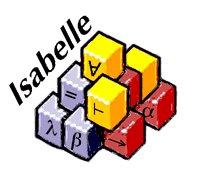
\includegraphics[scale=0.5]{images/isabelle.png}

\begin{itemize}
\item{Isabelle/HOL es un demostrador interactivo de teoremas escrito en ML.}
\pause
\item{Desarrollado por Larry Paulson y Tobias Nipkow.}
\pause
\item{Utiliza el lenguaje HOL para realizar las pruebas.}
\pause
\item{Permite hacer definiciones y demostrar propiedades acerca de las mismas.}
\pause
\item{Se usa la máquina para asistir en las demostraciones}
\pause
\end{itemize}

\end{frame}

\begin{frame}
\frametitle{Ejemplo de una prueba en Isabelle/HOL}

\begin{semiverbatim}
datatype \textit{nat} = 0 | Suc \textit{nat}


fun add :: ``nat => nat => nat'' where

\alert<2>{``add 0 n = n''} |

\alert<4>{``add (Suc m) n = Suc (add m n)''}
\end{semiverbatim}

\begin{columns}[t]
\column{.45\textwidth}
\begin{semiverbatim}
\only<1,2,3,4,5>{
lemma add\_02:

``add m 0 = m''

proof(induction)}
\only<2,3,4,5>{
\alert<2>{

apply simp}
}
\only<4,5>{
\alert<4>{

apply simp}

done
}
\end{semiverbatim}
\column{.45\textwidth}
\begin{block}{Output de Isabelle}
\begin{semiverbatim}
\only<1,2>{
\alert<2>{
1. add 0 0 = 0}

}

\only<1,2,3,4>{
\alert<4>{
2. $\bigwedge$ m. add m 0 = m $\Longrightarrow$

add (Suc m) 0 = Suc m
}}
\only<5>{

No subgoals!
}
\end{semiverbatim}
\end{block}
\end{columns}

\only<2>{
\bigskip

Usando la primera regla de add}
\only<4>{
\bigskip

Usando la segunda regla de add y luego la hipotesis inductiva}

\end{frame}

\begin{comment}

\end{comment}

\section{Antecedentes}


\begin{frame}
\frametitle{Antecedentes}
\framesubtitle{Michael Norrish: Semántica de C formalizada en HOL}

\begin{itemize}
\item{Semántica operacional de pasos largos para el subconjunto Cholera de C en HOL.}
\item{Considera todo posible orden de evaluación para efectos de borde.}
\item{Deriva una lógica de Hoare para programas en C.}
\item{Sistema para analizar cuerpos de ciclos y generar postcondiciones correctas.}
\end{itemize}


\end{frame}


\begin{frame}
\frametitle{Antecedentes}
\framesubtitle{Proyecto CompCert}

\begin{itemize}
\item{Compilador moderadamente optimizador}
\item{Traduce código del subconjunto Clight de C a código ensamblador para PowerPC.}
\item{Modelo de memoria interesante para lenguajes imperativos.}
\item{Formalización y demostración de propiedades en operaciones de memoria usando Coq.}
\end{itemize}


\end{frame}


\begin{frame}
\frametitle{Antecedentes}
\framesubtitle{Proyecto AutoCorres}

\begin{itemize}
\item{Enfoque \textit{bottom-up}}
\item{Reconoce lexicográficamente código C y genera una representación monádica de más alto nivel.}
\item{Esta representación generada facilita el razonamiento sobre programas.}
\item{Se utiliza en varios proyectos de verificación de C:}
\begin{itemize}
\item{Verificación de una libería de grafos a gran escala}
\item{Verificación de un sistema de archivos}
\item{Verificación de un sistema operativo de tiempo real}
\end{itemize}
\end{itemize}


\end{frame}

\section{Sintaxis y semántica}

\begin{frame}[fragile]
\frametitle{¿Qué es un programa?}

Un programa es una secuencia de una o mas instrucciones que realizan una tarea en una computadora:

\begin{example}
\begin{semiverbatim}
x = 21;
y = 21;
z = x + y;
\end{semiverbatim}
\end{example}


\end{frame}

\subsection{Expresiones}

\begin{frame}[fragile]
\frametitle{Sintaxis}
\framesubtitle{Expresiones en Chloe}

\begin{columns}[t]
\column{.45\textwidth}
\begin{semiverbatim}
\textbf{type_synonym} \textit{vname} = string

\textbf{datatype} \textit{exp} = Const \textit{int}
  | Null
  | V      \textit{vname}
  | Plus  \textit{exp} \textit{exp}
  | Subst \textit{exp} \textit{exp}
  | Minus \textit{exp}
  | Div   \textit{exp} \textit{exp}
  | Mod   \textit{exp} \textit{exp}
  | Mult  \textit{exp} \textit{exp}
  | Less  \textit{exp} \textit{exp}
  | Not   \textit{exp}
\end{semiverbatim}
\column{.45\textwidth}
\begin{semiverbatim}
  | And   \textit{exp} \textit{exp}
  | Or    \textit{exp} \textit{exp}
  | Eq    \textit{exp} \textit{exp}
  | New   \textit{exp}
  | Deref \textit{exp}
  | Ref   \textit{lexp}
  | Index \textit{exp} \textit{exp}
and
\textbf{datatype} \textit{lexp} = Deref \textit{exp}
  | Indexl \textit{exp} \textit{exp}
\end{semiverbatim}
\end{columns}


\end{frame}


\begin{frame}[fragile]
\frametitle{Sintaxis}
\framesubtitle{Expresiones en Chloe}

¿Por qué diferenciamos entre \textit{exp} y \textit{lexp}?
\begin{example}
\begin{semiverbatim}
foo = *bar;
*baz = 1;
\end{semiverbatim}
\end{example}



\end{frame}


\begin{frame}[fragile]
\frametitle{Tipos}
\framesubtitle{Enteros y apuntadores}

Los enteros son palabras de precisión 64.
\begin{block}{}
\begin{semiverbatim}
\textbf{type_synonym} int_width = 64
\textbf{type_synonym} int_val = int_width word
\end{semiverbatim}
\end{block}
Y tienen los siguientes límites:
\begin{block}{}
\begin{semiverbatim}
INT_MIN == - (2^(int_width - 1))
INT_MAX ==  ((2^(int_width - 1)) - 1)
\end{semiverbatim}
\end{block}

Un apuntador es un par que representa un identificador de un bloque y un desplazamiento.

\end{frame}


\begin{frame}[fragile]
\frametitle{Memoria dinámica}
\framesubtitle{Diseño del \textit{heap}}


\begin{columns}[t]
\column{.45\textwidth}
\begin{block}{Ejemplo de memoria}
\begin{tikzpicture}
\alert<2>{\draw (0,0) rectangle (5,2); }
\alert<3>{\draw (0,-1) rectangle (5,0) node[midway] {None};}
\alert<4>{\draw (0.25,0.25) rectangle (0.75,1.75) node[midway] {21};}
\draw (0.75,0.25) rectangle (2.25,1.75) node[midway] {NullVal};
\alert<5>{\draw (2.25,0.25) rectangle (3.75,1.75) node[midway] {None};}
\draw (3.75,0.25) rectangle (4.25,1.75) node[midway] {12};
\end{tikzpicture}
\end{block}
\column{.45\textwidth}
\begin{itemize}
\alert<2>{\item{Bloque asignado}}
\alert<3>{\item{Bloque Libre}}
\alert<4>{\item{Celda inicializada}}
\alert<5>{\item{Celda no inicializada}}
\end{itemize}
\end{columns}


\end{frame}


\begin{comment}
\begin{frame}[fragile]
\frametitle{Memoria dinámica}
\framesubtitle{Operaciones de manejo de memoria}

\begin{itemize}
\item<1-3>{new\_block :: $val\ \Rightarrow\ mem\ \Rightarrow\ (val\ \times\ mem)$ option}
\item<1,2,4>{free :: $addr\ \Rightarrow\ visible\_state\ \Rightarrow\ visible\_state$ option}
\item<1,2,5>{load :: $addr\ \Rightarrow\ mem\ \Rightarrow\ val$ option}
\item<1,2,6>{store :: $addr\ \Rightarrow\ val\ \Rightarrow\ visible\_state\ \Rightarrow\ visible\_state$ option}
\end{itemize}

\alert<2>{Los tipos de retorno son $\tau$ option, ya que las funciones siempre pueden fallar.}

\end{frame}
\end{comment}


\begin{frame}[fragile]
\frametitle{Problema de la memoria ilimitada}
\framesubtitle{Soluciones posibles}

La asignación de memoria no puede fallar porque se supone una cantidad ilimitada de memoria.

\bigskip

Sin embargo, se tienen recursos limitados en una computadora.

Hay dos soluciones posibles:

\begin{itemize}
\item{Modelar un comportamiento no-determinístico en la función que asigna memoria.}
\item{Suponer una cantidad fija de memoria.}
\end{itemize}


\end{frame}


\begin{frame}
\frametitle{Problema de la memoria ilimitada}
\framesubtitle{Nuestra solución}

Se mantiene la suposición de memoria ilimitada.

\bigskip
Luego en el proceso de traducción se envuelve la función malloc de C en una definida por nosotros.

\bigskip
Esta función verifica si la llamada a malloc falla.

\bigskip
Si falla, entonces el programa se aborta.


\end{frame}


\begin{frame}
\frametitle{Semántica de las expresiones}
\framesubtitle{¿Cuál es el significado de una expresión?}

La semántica de una expresión es su valor y efecto en el estado del programa.

\pause
\begin{example}
$21 + 21 = 42$

\pause

$foo + 42 = ?$

\pause

$bar = new (12)$
\end{example}
\pause

Se debe saber el valor de una variable a tiempo de ejecución.



\end{frame}


\begin{frame}[fragile]
\frametitle{Semántica de las expresiones}
\framesubtitle{Valuaciones}

Una valuación es una función que mapea un nombre de variable a un valor.

\bigskip
\pause

\textbf{type\_synonym} valuation = vname $\Rightarrow$ val option option

\bigskip

\pause
Dado un nombre de variable puede producir tres resultados diferentes:

\bigskip

\pause
\begin{itemize}
\item{None: valor sin definir.}
\pause
\item{Some None: valor sin inizializar.}
\pause
\item{Some $v$: variable inicializada que tiene valor $v$.}
\end{itemize}


\end{frame}


\begin{frame}
\frametitle{Semántica de las expresiones}
\framesubtitle{Estado visible}

Cuando se ejecuta un comando, el mismo solo puede \textit{ver} cierta parte del estado:

\bigskip
\pause
\begin{itemize}
\item{Variables locales a la función actual}
\pause
\item{Variables globales}
\pause
\item{Memoria}
\end{itemize}


\end{frame}


\begin{frame}
\frametitle{Semántica de las expresiones}
\framesubtitle{Funcioness eval y eval\_l}

Se definen dos funciones para calcular el valor de una expresión.

\bigskip

La evaluación de estas funciones puede fallar:

\bigskip
\pause

\begin{itemize}
\item{Variables sin definir}
\pause
\item{Operandos ilegales dados a la función}
\pause
\item{Acceso a memoria inválida}
\pause
\item{\textit{Overflow} de enteros}
\pause
\item{División por cero}
\end{itemize}


\end{frame}


\begin{frame}
\frametitle{Semántica de las expresiones}
\framesubtitle{Highlights of expression evaluation}
\framesubtitle{Aspectos destacados de la evaluación de expresiones}

\begin{itemize}
\item{Se detecta \textit{overflow} de enteros y lleva a un estado erróneo}
\item{Evaluación de corto circuito}
\item{División y módulo con truncamiento a cero}
\item{Alcance estático de las variables}
\end{itemize}


\end{frame}


\subsection{Comandos}


\begin{comment}
\begin{frame}[fragile]
\frametitle{Syntax of commands}
\framesubtitle{Concrete syntax}

\begin{semiverbatim}
com ::= SKIP
     | lexp ::== exp
     | vname ::= exp
     | com ;; com
     | IF exp THEN com ELSE com
     | WHILE exp DO com
     | FREE lexp
     | RETURN exp
     | RETURNV
     | lexp ::== f ( [exp] )
     | vname ::= f ( [exp] )
     | CALL f ( [exp])
\end{semiverbatim}


\end{frame}
\end{comment}


\begin{frame}[fragile]
\frametitle{Sintaxis de los comandos}
\framesubtitle{Sintaxis Abstracta}

\begin{semiverbatim}
\textbf{datatype} com = SKIP
             | Assignl lexp exp
             | Assign  vname exp
             | Seq     com  com
             | If      exp com com
             | While   exp com
             | Free    lexp
             | Return exp
             | Returnv
             | Callfunl lexp fname " exp list"
             | Callfun vname fname " exp list"
             | Callfunv fname " exp list"
\end{semiverbatim}

\end{frame}


\begin{frame}[fragile]
\frametitle{Funciones}
\framesubtitle{}

Se tienen funciones que retornan un valor y aquellas que no.

\begin{semiverbatim}
\textbf{record} fun_decl =
  name :: fname
  params :: vname list
  locals :: vname list
  body :: com
\end{semiverbatim}

\bigskip

Una función es válida $\Longleftrightarrow$ los parámetros y variables locales tienen nombres diferentes.

\bigskip

Cuando una función retorna un valor, este valor es:

\begin{itemize}
\item{Asignado a una ubicación en memoria}
\item{Asignado a una variable}
\item{Ignorado}
\end{itemize}


\end{frame}


\begin{frame}[fragile]
\frametitle{Programas}

\begin{semiverbatim}
\textbf{record} program =
  name :: fname
  globals :: vname list
  procs :: fun_decl list
\end{semiverbatim}
\pause

\begin{block}{Un programa se considera válido si:}
\begin{itemize}
\item{Las variables globales tienen nombres diferentes entre sí.}
\pause
\item{Los nombres de funciones son dieferentes entre sí.}
\pause
\item{Todas las declaraciones de funciones son válidas.}
\pause
\item{La función main está definida.}
\pause
\item{Ninguno de los nombres de variables o funciones en el programa es una palabra reservada.}
\pause
\item{Los nombres de variables globales y funciones son diferentes entre sí.}
\end{itemize}
\end{block}


\end{frame}


\begin{frame}[fragile]
\frametitle{Pila de ejecución}
\framesubtitle{Ubicaciones de retorno y marcos de pila}

\begin{semiverbatim}
\textbf{datatype} return_loc = \alert<3>{Ar \textit{addr}} | \alert<4>{Vr \textit{vname}} | \alert<5>{Invalid}
\end{semiverbatim}

\pause

Un valor de retorno de una función puede ser:
\begin{itemize}
\item<3->{\alert<3>{Asignado a una ubicación en memoria}}
\item<4->{\alert<4>{Asignado a una variable}}
\item<5->{\alert<5>{Ignorado}}
\end{itemize}


\bigskip
\onslide<6->{\textbf{datatype} stack\_frame = com $\times$ valuation $\times$ return\_loc}

\bigskip

\onslide<6>{The execution stack is a list of stack frames.}


\end{frame}


\begin{frame}[fragile]
\frametitle{Pila de ejecución}
\framesubtitle{Convención de llamada}

\only<2,4>{
\begin{drawstack}[baseline=(current bounding box.north), scale=0.8]
  \only<2>{
  \startframe
  \cell{x=sum(2,2)}
  \cell{[x$\mapsto$0]}
  \cell{Invalid}
  \finishframe{main}}
  \only<4>{
  \startframe
  \cell{return a+b}
  \cell{[a$\mapsto$2, b$\mapsto$2]}
  \alert<4>{\cell{Invalid}}
  \finishframe{sum}
  \startframe
  \cell{x=sum(2,2)}
  \cell{[x$\mapsto$0]}
  \alert<4>{\cell{x}\only<4>{\cellround{Caller's rloc changes!}}}
  \finishframe{main}
  }
\end{drawstack}
}

\begin{semiverbatim}
\only<1,3>{
int sum(int a; int b){
  return a+b;
}

int main(){
  int x = 0;
  \alert<3>{x = sum(2,2);}
}
}
\end{semiverbatim}


\end{frame}

\subsection{Estados}

\begin{frame}
\frametitle{Tabla de procedimientos y estados}
\framesubtitle{}

La tabla de procedimientos mapea nombres de funciones a sus declaraciones:
\bigskip

\textbf{type\_synonym} proc\_table = fname $\rightharpoonup$ fun\_decl
\pause
\bigskip

Se construye juntando cada declaración de función con su nombre.

\pause
\bigskip

Un estado se define como:
\bigskip
\pause

\textbf{type\_synonym} state = stack\_frame list $\times$ valuation $\times$ mem

\pause

\begin{itemize}
\item{Pila de ejecución}
\item{Variables globales}
\item{Memoria}
\end{itemize}

\end{frame}


\begin{frame}
\frametitle{Estados}
\framesubtitle{Estado inicial}

Un estado inicial es la tupla que contiene:

\begin{itemize}
\item{Pila inicial: Pila de ejecución con el marco de pila de la función main}
\item{Variables globales iniciales: todos los nombres de variables se mapean a indefinido y las varaibles globales a no-inicializado}
\item{Memoria inicial: Memoria vacía}
\end{itemize}


\end{frame}


\subsection{Semántica de pasos cortos}


\begin{frame}[fragile]
\frametitle{Grafo de flujo de control}
\framesubtitle{¿Qué es un CFG?}

Una representación en forma de grafo que cubre los diferentes caminos que un programa puede tomar durante su ejecución.


\begin{figure}
\centering
\tikzstyle{cfg_node} = [circle, draw, fill=uablue25, 
    text width=2em, text centered, minimum height=1em, line width=1pt ]
\tikzstyle{line} = [line width=1pt, -triangle 45]
\tikzstyle{alert} = [text=uared100, fill=uared25, draw=uared100]
\tikzstyle{alert_pp} = [text=uared100]
\tikzstyle{dim} = [text=uablue25, fill=uablue5, draw=uablue25]

\begin{tikzpicture}[node distance=1.5cm, auto]
    % Place nodes
    \node [cfg_node,onslide=<2>{alert}] (c1) {$c_1$};
    \node [cfg_node,onslide=<2>{alert}] (c2) [right of=c1, node distance=3cm] {$c_2$};
    \node [onslide=<6>{alert_pp}](pp) [above left of=c1, node distance=1.5cm] {program pointer};
    %\node [block,onslide=<2->{dim}] (client) {Web Client};
    %\node [block,onslide=<2->{dim}] (python) [right of=client, node distance=3cm] {Python Service};
    %\node [block,onslide=<2->{dim}] (wavefront) [right of=python, node distance=3cm] {Wavefront};
    %\node [block,onslide=<2->{dim}] (AMCL) [above of=wavefront] {AMCL};
    %\node [block,temporal=<2>{}{alert}{dim}] (VFH) [below of=wavefront] {VFH};
    %\node [block,onslide=<2->{dim}] (laser) [above right=0.5cm and 1.2cm of AMCL] {Laser};
    %\node [block,onslide=<2->{dim}] (dash7) [right of=AMCL, node distance=3cm] {DASH7};
    %\node [block,onslide=<2->{dim},temporal=<3>{}{alert}{dim}] (robot) [right of=wavefront, node distance=3cm] {Robot};
    % Draw edges
    \draw [line,onslide=<3-5>{alert}] (c1) node[above right of=c1, node distance=1.25cm] {(en, tr)} -> (c2);
    \draw [line,onslide=<6>{alert}] (pp) -> (c1);
    %\draw [line] (client.east) -> (python.west);
    %\draw [line] (python) -> (client);
    %\draw [line] (python) -- (wavefront);
    %\draw [line] (AMCL) -- (wavefront);
    %\draw [line] (AMCL) edge[out=180,in=90] (python);
    %\draw [line] (python) edge[out=270,in=180] (VFH);
    %\draw [line] (wavefront) -- (VFH);
    %\draw [line] (laser) -> (AMCL);
    %\draw [line] (dash7) -> (AMCL);
    %\draw [line] (robot) -> (AMCL);
    %\draw [line] (VFH) edge[out=0,in=270] (robot);
\end{tikzpicture}
\end{figure}


\begin{itemize}
\item<2->{Los nodos del CFG son comandos}
\item<3->{Las aristas del CFG están anotadas con dos funciones que dependen del estado del programa}
  \begin{itemize}
  \item<4->{La primera indica si una arista puede ser seguida o no}
  \item<5->{La segunda indica como se transforma el estado al seguir una arista}
  \end{itemize}
 \item<6->{Se tiene una ubicación actual, la cual es un \textit{program pointer} al nodo actual}
\end{itemize}


\end{frame}


\begin{frame}
\frametitle{Grafo de flujo de control}
\framesubtitle{Funciones \textit{enabled}}

\begin{figure}[fragile]
\centering
\tikzstyle{cfg_node} = [circle, draw, fill=uablue25, 
    text width=2em, text centered, minimum height=1em, line width=1pt ]
\tikzstyle{cfg_big_node} = [circle, draw, fill=uablue25, 
    text width=4.5em, text centered, minimum height=2.25em, line width=1pt ]
\tikzstyle{line} = [line width=1pt, -triangle 45]
\tikzstyle{alert} = [text=uared100, fill=uared25, draw=uared100]
\tikzstyle{alert_pp} = [text=uared100]
\tikzstyle{dim} = [text=uablue25, fill=uablue5, draw=uablue25]

\begin{block}{}
\textbf{type\_synonym} enabled = state $\rightharpoonup$ bool
\end{block}

\bigskip


\begin{tikzpicture}[node distance=1.5cm, auto]
    % Place nodes
    \node [cfg_big_node,onslide=<1>{dim},onslide=<2-3>{alert}] (if) {IF $b$ THEN $c_1$ ELSE $c_2$};
    \node [cfg_node,onslide=<1>{dim},onslide=<2>{alert}] (c1) [right of=if, node distance=4cm] {$c_1$};
    \node [cfg_node,onslide=<1-2>{dim},onslide=<3>{alert}] (c2) [left of=if, node distance=4cm] {$c_2$};
    %\node [block,onslide=<2->{dim}] (client) {Web Client};
    %\node [block,onslide=<2->{dim}] (python) [right of=client, node distance=3cm] {Python Service};
    %\node [block,onslide=<2->{dim}] (wavefront) [right of=python, node distance=3cm] {Wavefront};
    %\node [block,onslide=<2->{dim}] (AMCL) [above of=wavefront] {AMCL};
    %\node [block,temporal=<2>{}{alert}{dim}] (VFH) [below of=wavefront] {VFH};
    %\node [block,onslide=<2->{dim}] (laser) [above right=0.5cm and 1.2cm of AMCL] {Laser};
    %\node [block,onslide=<2->{dim}] (dash7) [right of=AMCL, node distance=3cm] {DASH7};
    %\node [block,onslide=<2->{dim},temporal=<3>{}{alert}{dim}] (robot) [right of=wavefront, node distance=3cm] {Robot};
    % Draw edges
    \draw [line,onslide=<2>{alert}] (if) node[above left of=c1, node distance=1.5cm] {(en\_pos, tr)} -> (c1);
    \draw [line,onslide=<3>{alert}] (if) node[above right of=c2, node distance=1.5cm] {(en\_neg, tr)} -> (c2);
    %\draw [line] (client.east) -> (python.west);
    %\draw [line] (python) -> (client);
    %\draw [line] (python) -- (wavefront);
    %\draw [line] (AMCL) -- (wavefront);
    %\draw [line] (AMCL) edge[out=180,in=90] (python);
    %\draw [line] (python) edge[out=270,in=180] (VFH);
    %\draw [line] (wavefront) -- (VFH);
    %\draw [line] (laser) -> (AMCL);
    %\draw [line] (dash7) -> (AMCL);
    %\draw [line] (robot) -> (AMCL);
    %\draw [line] (VFH) edge[out=0,in=270] (robot);
\end{tikzpicture}
\end{figure}

\only<1>{Esta función indica si un estado puede continuar su ejecución.

Es una función parcial, por lo que puede fallar.}

\only<2>{Cuando la evaluación de la condición b produce un valor true, se sigue la arista que lleva a $c_1$.}

\only<3>{Cuando la evaluación de la condición b produce un valor false, se sigue la arista que lleva a $c_2$.}

\only<4>{Dependiendo del resultado de la función \textit{enabled} se decide que arista tomar.}

\only<5>{Siempre habrá una arista que pueda ser seguida.}

\end{frame}


\begin{frame}
\frametitle{Grafo de flujo de control}
\framesubtitle{Funciones \textit{transformer}}

\begin{block}{}
\textbf{type\_synonym} transformer = state $\rightharpoonup$ state
\end{block}
\bigskip

Esta función transforma un estado en uno nuevo dependiendo de la arista que se siga.

\bigskip

Es una función paracial, falla cuando se encuentra un error en la transformación.

\bigskip

Esta función actualiza el estado con el estado resultante cada vez que se sigue una arista.



\end{frame}


\begin{comment}
\begin{frame}
\frametitle{Control Flow Graph}
\framesubtitle{How do our transformer functions behave?}

\only<1>{We have a set of functions that will take the neccessary parameters to yield an appropiate transformer function for each command in Chloe.}

\pause
\begin{itemize}
\item\only<2->{{\textbf{tr\_id} :: transformer where tr\_id $\equiv$ Some}}
\item\only<3->{{\textbf{tr\_assign} :: vname $\Rightarrow$ exp $\Rightarrow$ transformer}}
\item\only<4->{{\textbf{tr\_assignl} :: lexp $\Rightarrow$ exp $\Rightarrow$ transformer}}
\item\only<5->{{\textbf{tr\_eval} :: exp $\Rightarrow$ transformer}}
\item\only<6->{{\textbf{tr\_free} :: lexp $\Rightarrow$ transformer}}
\item\only<7->{{\textbf{call\_function} :: proc\_table $\Rightarrow$ fname $\Rightarrow$ exp list $\Rightarrow$ transformer}}
\item\only<8->{{\textbf{tr\_callfunl} :: proc\_table $\Rightarrow$ lexp $\Rightarrow$ fname $\Rightarrow$ exp list $\Rightarrow$ transformer}}
\item\only<9->{{\textbf{tr\_callfun} :: proc\_table $\Rightarrow$ vname $\Rightarrow$ fname $\Rightarrow$ exp list $\Rightarrow$ transformer}}
\item\only<10->{{\textbf{tr\_callfunv} :: proc\_table $\Rightarrow$ fname $\Rightarrow$ exp list $\Rightarrow$ transformer}}
\item\only<11->{{\textbf{tr\_return} :: exp $\Rightarrow$ transformer}}
\item\only<12->{{\textbf{tr\_return\_void} :: transformer}}
\end{itemize}

\end{frame}
\end{comment}


\begin{frame}[fragile]
\frametitle{Grafo de control de flujo}
\framesubtitle{\ldots con una pila.}

\begin{figure}
\centering
\tikzstyle{cfg_node} = [circle, draw, fill=uablue25, 
    text width=1em, text centered, minimum height=1em, line width=1pt ]
\tikzstyle{line} = [line width=1pt, -triangle 45]
\tikzstyle{alert} = [text=uared100, fill=uared25, draw=uared100]
\tikzstyle{alert_pp} = [text=uared100]
\tikzstyle{dim} = [text=uablue25, fill=uablue5, draw=uablue25]

\begin{tikzpicture}[node distance=1.5cm, auto, baseline=(current bounding box.north)]
    % Place nodes
    \node [cfg_node] (c1) {$f()$};
    \node [cfg_node] (c2) [right of=c1, node distance=3cm] {$c_2$};
    \node (pp) [above left of=c1, node distance=1.5cm] {program pointer};
    \node (pp3) [above left of=c2, node distance=1.5cm] {program pointer};

    \node [cfg_node] (c3) [below of=c1, node distance=3cm] {$c_3$};
    \node (pp2) [above left of=c3, node distance=1.5cm] {f()};
    \node [cfg_node] (c4) [right of=c3, node distance=1.5cm] {$c_4$};
    \node [cfg_node] (c5) [right of=c4, node distance=1.5cm] {$c_5$};
    % Draw edges
    \draw [line] (c1) -> (c2);
    \draw [line] (c3) -> (c4);
    \draw [line] (c4) -> (c5);
    \draw [line,onslide=<2->{dim}] (pp) -> (c1);
    \draw [line,onslide=<2>{alert},onslide=<3->{dim},onslide=<1>{dim}] (pp3) -> (c2);
    \draw [line,onslide=<3>{alert},onslide=<1-2>{dim}] (pp2) -> (c3);
\end{tikzpicture}
\end{figure}

\begin{tikzpicture}[stack/.style={rectangle split, rectangle split parts=#1,draw, anchor=center}, baseline=(current bounding box.north)]
\only<2>{
\node[stack=3]{
\nodepart{three}$c_2$
};
}

\only<3->{
\node[stack=3]{
\nodepart{two}$f()$
\nodepart{three}$c_2$
};
}
\end{tikzpicture}


\end{frame}


\begin{frame}[fragile]
\frametitle{Grafo de flujo de control}
\framesubtitle{Reglas}

\textbf{type\_synonym} cfg\_label = enabled $\times$ transformer

\bigskip

\textbf{inductive} cfg :: com $\Rightarrow$ cfg\_label $\Rightarrow$ com $\Rightarrow$ bool

\begin{itemize}
\item{Assign: \textbf{cfg} ($x$ ::= $a$) (en\_always,tr\_assign $x$ $a$) SKIP}
\item{Assignl: \textbf{cfg} ($x$ ::==  $a$) (en\_always,tr\_assignl $x$ $a$) SKIP}
\item{Seq1: \textbf{cfg} (SKIP;; $c_{2}$) (en\_always, tr\_id) $c_{2}$}
\item{Seq2: $[\![$\textbf{cfg} $c_{1}$ $a$ $c_{1}'$ $]\!]$ $\Longrightarrow$ \textbf{cfg} ($c_{1}$;; $c_{2}$) $a$ ($c_{1}'$;; $c_{2}$)}
\item{IfTrue: \textbf{cfg} (IF $b$ THEN $c_{1}$ ELSE $c_{2}$) (en\_pos $b$, tr\_eval $b$) $c_{1}$}
\item{IfFalse: \textbf{cfg} (IF $b$ THEN $c_{1}$ ELSE $c_{2}$) (en\_neg $b$, tr\_eval $b$) $c_{2}$}
\item{While: \textbf{cfg} (WHILE $b$ DO $c$) (en\_always, tr\_id)
  (IF $b$ THEN $c$;; WHILE $b$ DO $c$ ELSE SKIP)}
\item{Free: \textbf{cfg} (FREE $x$) (en\_always, tr\_free $x$) SKIP}
\end{itemize}

\end{frame}


\begin{frame}[fragile]
\frametitle{Grafo de flujo de control}
\framesubtitle{Reglas}

\begin{itemize}
\item{Return: \textbf{cfg} (Return $a$) (en\_always, tr\_return $a$) SKIP}
\item{Returnv: \textbf{cfg} Returnv (en\_always, tr\_return\_void) SKIP}

\item{Callfunl: \textbf{cfg} (Callfunl $e$ $f$ params)
  (en\_always, tr\_callfunl proc\_table $e$ $f$ params) SKIP}
\item{Callfun: \textbf{cfg} (Callfun $x$ $f$ params)
  (en\_always, tr\_callfun proc\_table $x$ $f$ params) SKIP}
\item{Callfunv: \textbf{cfg} (Callfunv $f$ params)
  (en\_always, tr\_callfunv proc\_table $f$ params) SKIP}
\end{itemize}

\end{frame}


\begin{frame}
\frametitle{Semántica de pasos cortos}
\framesubtitle{}

¿Por qué una semántica de pasos cortos?
\bigskip
\pause

Se quiere poder hablar de estados intermedios y diferenciar entre programas que no terminen y programas erróneos.

\bigskip
\pause


\begin{block}{La semántica de pasos cortos se define sobre estados:}
\textbf{inductive} small\_step :: state $\Rightarrow$ state option $\Rightarrow$ bool
\bigskip

$s\ \rightarrow\ s_2$

$\equiv$

``Se toma un paso corto desde $s$ hasta $s_2$''
\end{block}


\end{frame}


\begin{frame}
\frametitle{Semántica de pasos cortos}
\framesubtitle{¿Cuándo se puede dar un paso?}

Un paso desde $s$ hasta $s_2$ se puede dar cuando:
\begin{itemize}
\item{Paso regular:}
\begin{itemize}
\item{Pila no vacía}
\item{Hay una arista en el CFG entre $c_1$ y $c_2$}
\item{El comando en el tope de la pila es $c_1$}
\item{Aplicar la función enabled produce True}
\item{Aplicar la función transformer sobre $s$ produce $s_2$}
\end{itemize}
\item{Paso de retorno desde una función sin valor de retorno:}
\begin{itemize}
\item{Pila no vacía}
\item{El comando en el tope de la pila es SKIP}
\item{Aplicar la función transformer tr\_return\_void sobre $s$ produce $s_2$}
\end{itemize}
\end{itemize}

\end{frame}


\begin{frame}
\frametitle{Semántica de pasos cortos}
\framesubtitle{¿Cuándo falla el dar un paso?}

Cuando hay una ejecución errónea, se da un paso desde $s$ a None:
\begin{itemize}
\item{Paso regular:}
\begin{itemize}
\item{Pila no vacía}
\item{Hay una arista en el CFG entre $c_1$ y $c_2$}
\item{El comando en el tope de la pila es $c_1$}
\item{Aplicar la función enabled o transformer produce None}
\end{itemize}
\item{Paso de retorno desde una función sin valor de retorno:}
\begin{itemize}
\item{Pila no vacía}
\item{El comando en el tope de la pila es SKIP}
\item{Aplicar la función transformer tr\_return\_void sobre $s$ produce None}
\end{itemize}
\end{itemize}


\end{frame}


\begin{frame}
\frametitle{Semántica de pasos cortos}
\framesubtitle{¿Cómo dar varios pasos cortos?}

Se lleva la definicón de small\_step a trabajar sobre state option:

\bigskip
\textbf{inductive} small\_step' :: state option $\Rightarrow$ state option $\Rightarrow$ bool
\bigskip
\pause

Para tomar varios pasos se utiliza la clausura reflexivo-transitiva sobre small\_step':

\bigskip
\textbf{inductive} small\_step' :: state option $\Rightarrow$ state option $\Rightarrow$ bool
\bigskip

$s\ \rightarrow*\ s_2$

$\equiv$

``Se toma uno o mas pasos cortos desde $s$ hasta $s_2$''



\end{frame}


\subsection{Interpretador}


\begin{frame}
\frametitle{Interpretador}
\framesubtitle{Ejecución de un programa}

Un paso se ejecuta al aplicar la función \textit{transformer} correspondiente al estado y actualizar el comando en el tope de la pila.
\bigskip
\pause

La semántica es determinística, lo que permite escribir un interpretador para la misma.
\bigskip
\pause

\begin{block}{Interpretar un programa:}
Mientras no se alcance un estado final, se ejecuta un paso.
\end{block}

\pause

\begin{block}{Ejecutar un programa:}
Verificar que el programa es válido.

Si lo es, se interpreta.
\end{block}

\bigskip

El interpretador retorna un estado final o None, que indica una ejecución errónea.

\end{frame}

\begin{frame}[fragile]
\frametitle{Correctitud}
\Fontvi

Se demuestran varias propiedades con respecto a la semántica y el interpretador con asistencia de Isabelle/HOL.

Tomemos como ejemplo la prueba del siguiente teorema:



\begin{columns}[t]
\column{.45\textwidth}
\begin{semiverbatim}
lemma cfg_has_enabled_action:
  assumes " c \\notequal SKIP"
  shows "\\exists c' en tr. cfg c (en,tr) c'
    \\and (en s = None \\or en s = Some True)" 
  using assms
proof (induction c)
  case (Seq c1 c2)
  show ?case
  proof (cases "c1 = SKIP")
    case True
    thus ?thesis by (auto intro: cfg.intros)
  next
    case False
    from Seq.IH(1)[OF this]
      show ?thesis by (auto intro: cfg.intros)
  qed
next
\end{semiverbatim}
\column{.45\textwidth}
\begin{semiverbatim}
  case (If b c1 c2)
  show ?case
  proof (cases "en_pos b s")
    case None[simp]
    thus ?thesis
      by (fastforce intro: cfg.intros)
  next
    case (Some a)[simp]
      show ?thesis
      proof (cases a)
        case True
        thus ?thesis
          by (fastforce intro: cfg.intros)
      next
        case False[simp]
        have "en_pos b s = Some False" by simp
        hence "en_neg b s = Some True"
          unfolding en_pos_def en_neg_def
          by (auto split: Option.bind_splits)
        thus ?thesis
          by (fastforce intro: cfg.intros)
      qed
  qed
qed (auto intro: cfg.intros)
\end{semiverbatim}

\end{columns}


\end{frame}

\begin{frame}
\frametitle{Correctitud}

Se demuestran dos principales teoremas.

\begin{theorem}[La semántica es determinística]
$s \rightarrow s' \land s \rightarrow s'' \Longrightarrow s' = s''$

$s \rightarrow' s' \land s \rightarrow' s'' \Longrightarrow s' = s''$
\end{theorem}

Para demostrar estos dos lemas fue necesario demostrar 9 lemas previos.


\begin{theorem}[El interpretador es correcto con respecto a la semántica]
$\mathtt{terminates}\ cs\ \Longrightarrow\ \mathtt{yields}\ cs\ cs'\ \longleftrightarrow\ (cs'\ =\ \mathtt{interp}\ \mathtt{proc\_table}\ cs)$
\end{theorem}

\end{frame}


\section{Pretty Printing}

\begin{frame}[fragile]
\frametitle{Pretty Printing}
\framesubtitle{Generación de código para factorial}
\Fontvi

Se toma el siguiente programa en la semántica:

\begin{columns}[t]
\column{.45\textwidth}
\begin{semiverbatim}
definition factorial_decl :: fun_decl
  where "factorial_decl ==
    ( fun_decl.name = fact,
      fun_decl.params = [n],
      fun_decl.locals = [r, i],
      fun_decl.body =
        r ::= (Const 1);;
        i ::= (Const 1);;
        (WHILE (Less (V i) (Plus (V n) (Const 1))) DO
          (r ::= (Mult (V r) (V i));;
          i ::= (Plus (V i) (Const 1)))
        );;
        RETURN (V r)
    )"

definition main_decl :: fun_decl
  where "main_decl ==
    ( fun_decl.name = main,
      fun_decl.params = [],
      fun_decl.locals = [],
      fun_decl.body =
        n ::= Const 5;;
        r ::= fact ([V n])
    )"
\end{semiverbatim}
\column{.45\textwidth}
\begin{semiverbatim}
definition p :: program
  where "p ==
    ( program.name = fact,
      program.globals = [n, r],
      program.procs = [factorial_decl, main_decl]
    )"
\end{semiverbatim}

y se exporta código para el mismo.
\end{columns}


\end{frame}


\begin{frame}[fragile]
\frametitle{Pretty Printing}
\framesubtitle{Generación de código para factorial}
\Fontvi

Se obtiene el siguiente código:

\begin{columns}[t]
\column{.65\textwidth}
\begin{semiverbatim}
\alert<2>{#include <stdlib.h>}
\alert<2>{#include <stdio.h>}
\alert<2>{#include <limits.h>}
\alert<2>{#include <stdint.h>}
\alert<2>{#include "../test_harness.h"}
\alert<2>{#include "../malloc_lib.h"}
\alert<3>{#ifndef INTPTR_MIN}
  \alert<3>{#error ("Macro INTPTR_MIN undefined")}
\alert<3>{#endif}
\alert<3>{#ifndef INTPTR_MAX}
  \alert<3>{#error ("Macro INTPTR_MAX undefined")}
\alert<3>{#endif}
\alert<3>{#if ( INTPTR_MIN + 1 != -9223372036854775807 )}
  \alert<3>{#error (" Assertion INTPTR_MIN + 1 == -9223372036854775807 failed")}
\alert<3>{#endif}
\alert<3>{#if ( INTPTR_MAX != 9223372036854775807 )}
  \alert<3>{#error (" Assertion INTPTR_MAX == 9223372036854775807 failed")}
\alert<3>{#endif}


\alert<4>{intptr_t n;}
\alert<4>{intptr_t r;}
\end{semiverbatim}
\column{.35\textwidth}
\begin{semiverbatim}
\alert<5>{intptr_t fact(intptr_t n) {}
\alert<5>{  intptr_t r;}
\alert<5>{  intptr_t i;}
\alert<5>{  r = (1);}
\alert<5>{  i = (1);}
\alert<5>{  while ((i) < ((n) + (1))) {}
\alert<5>{    r = ((r) * (i));}
\alert<5>{    i = ((i) + (1));}
\alert<5>{  }}
\alert<5>{  return(r);}
\alert<5>{}}

\alert<6>{intptr_t main() {}
\alert<6>{  n = (5);}
\alert<6>{  (r) = (fact(n));}
\alert<6>{}}
\end{semiverbatim}
\end{columns}


\end{frame}


\begin{frame}
\frametitle{Pretty Printing}
\framesubtitle{Casting}

Se traducen los programas usando el tipo intptr\_t de C.
\bigskip

Este tipo permite que tanto un apuntador como un entero se guarde en el.

Todas las variables se definen con el tipo ``intptr\_t''.

\bigskip

A veces se quiere que C interprete los valores como enteros y otras como apuntadores.

Se debe poder imprimir un \textit{cast} desde y hacia apuntadores.

\bigskip
\pause

\begin{block}{Casteo a apuntador}
(intptr\_t *) $<$expression$>$

*((intptr\_t *) foo);
\end{block}

\begin{block}{Casteo desde apuntador}
(intptr\_t) $<$expression$>$

(intptr\_t) \_\_MALLOC(sizeof(intptr\_t) * 5);
\end{block}


\end{frame}


\begin{frame}
\frametitle{Pretty Printing}
\framesubtitle{¿Cómo se traduce malloc bajo la suposición de memoria ilimitada?}

Se traduce malloc envolviendola en otra función.

\begin{block}{Generación de código para malloc}
New (Const $9$) se traduce como: \_\_MALLOC(sizeof(intptr\_t) * $9$)
\end{block}

\bigskip

Esta función abortará la ejecución del programa si encuentra un error de memoria.


\end{frame}


\begin{frame}
\frametitle{Exportando Código C}
\framesubtitle{Exportar a un archivo}

Se provee con un mecanismo que permite exportar el programa generado en código C a un archivo en un directorio determinado.


\end{frame}

\chapter{Testing}\label{chapter:testing}
\lhead{Capítulo 5. \emph{Testing}}

In chapters~\ref{chapter:semantics} and~\ref{chapter:pretty}, we have formalized the semantics for Chloe and described the translation process to C code.
Now we proceed to describe the testing process done to increase the trust in our translation process.
We guarantee that the code generated from our semantics will either end with an out of memory error or it will yield the same result as the same program executed in our semantics.
We say that the result of an execution of the semantics and the execution of the generated program in the machine is the same if the final states yielded by both are the same.
This means that we compute the final state yielded by our semantics and verify that after executing the generated program the state is the same i.e.\ the contents of the reachable memory and the global variables are the same.
When generating programs we can either simply generate the C code by itself or we can include a set of extra tests in the form of C macros that will guarantee what we mentioned before.

In the following sections we will proceed to describe the test harnesses used to generate tests for our code.
We will also give a more detailed description of the describe the meaning of the two final states being the same.
Finally, we will talk about a set of tests and example programs written in the semantics.
We only generate code for valid programs.
This means that we will go to an erroneous state if any undefined behavior arises.
In this set of tests we include programs which we expect to reach an erroneous state because they present undefined behavior or border cases.
For these \textit{incorrect} programs C code will not be generated.
We also present some example programs such as sorting algorithms to demonstrate how our semantics and code generation process work.


\section{Equality of final states}

We consider a final state yielded by the execution of our semantics equal to a final state of its generated C program, when, at the end of the execution, the values of the global variables are the same for both cases and every block of reachable memory has the same content.
We will now proceed to describe how we check for this equality between final states by the use of tests.

\subsection{Generation of Tests}

We can generate tests for our programs.
These will be executed at the end of the execution of the program and will test that the final state of the generated program is the same as the final state from the execution of the semantics.
We compare these final states by checking the values of global variables at the end of an execution against the ones in the final state of the execution of the semantics.

The direction in which the testing is done is by taking the values from the final state of the execution of the semantics and checking whether the execution of the generated code has the same values we expect it to have according to the execution of the semantics.

We will now introduce which kind of tests are done depending on whether the content of a global variable is an integer value or a pointer value.

\subsubsection{Integer Values}

When the content of a global variable we want to check is an integer value, we must simply generate a test that will check whether the integer value in the global variable at the end of the execution of the C code is the same value as the one we get from the global variables valuation in the final state of the execution of the semantics.

\subsubsection{Pointers}

With the checks for pointers we have two cases.
We have the null pointer and the non-null pointer case.

For null values we will generate a test, similar to the one for integer values, where we check if the content of the global variable is \verb|NULL|.

In the case of pointer values that are different from null, we will have a pointer to a block in the memory and we want to check if the content of that block in memory, at the end of the execution of the generated program, is the equal content of that same block in our final state in the semantics.
That complete block qualifies as reachable memory which is why we must check the content of each cell in the block.
For each cell in the block we will generate checks depending on what the expected content in the memory cell is, i.e\ an integer value, a null value or a pointer.

In the case of the pointer value checks, we will follow every pointer until we either reach an integer value or a pointer we already followed.
Upon reaching an integer value, we will generate an integer kind of test and upon reaching a pointer we already followed, we know that the path does not contain any pointer to invalid memory.
We check that the address for the beginning of the block is the same as the one we obtain from adjusting the pointer we followed to the beginning of the block.
In order to do this, we must follow pointers in a certain order and maintain a set of already \textit{discovered} blocks of memory.
This way when we find a pointer to a block of memory we already checked (or \textit{discovered}) we can stop and compare the pointer values instead of following the pointers in a cyclic manner indefinitely.

We present here the intuitive idea behind our tests generation and in the following sections we will describe the implementation details for the test harnesses, both in Isabelle and in C.

\section{Test Harness in Isabelle}

In this section we will introduce the Isabelle test harness that assists us in the generation of tests for our programs.
First, we define a new datatype for every kind of test instruction we can generate.
We can see this definition in figure~\ref{fig:test_harness_datatype}.


\begin{figure}
\begin{lstlisting}[mathescape=true]
datatype test_instr =
  Discover string nat
| Assert_Eq string int_val
| Assert_Eq_Null string
| Assert_Eq_Ptr string nat

fun adjust_addr :: "int $\Rightarrow$ string $\Rightarrow$ string"
  where
  "adjust_addr ofs ca = shows_binop (shows ca) (''-'') (shows ofs) ''''"

definition ofs_addr :: "int $\Rightarrow$ string $\Rightarrow$ string"
  where
  "ofs_addr ofs ca =
    (shows ''*'' o
      shows_paren (shows_binop (shows ca) (''+'') (shows ofs))) ''''"

definition base_var_name :: "nat $\Rightarrow$ string" where
  "base_var_name i $\equiv$ ''__test_harness_x_'' @ show i"
\end{lstlisting}

\caption{Definitions for the test harness}
\label{fig:test_harness_datatype}
\end{figure}

We have four different test instructions we can generate:

\begin{itemize}
  \item{\verb|Discover| represents an instruction that adds a block to the list of our \textit{discovered} blocks.
  The \verb|string| stands for the string representation of the expression in C and the \verb|nat| stands for the identification number of the current memory block.
  The actual addresses for the allocated memory blocks will vary with every execution of the program in the machine.
  The discover instruction pairs the actual address of a beginning of a block with the base block number to which it corresponds in our abstract representation.
  For this purpose we generate local variables with the function \verb|base_var_name| that are called \verb|__test_harness_x_|$n$ where $n$ represents the identification number for the block and in those variables we will save the actual address for the beginning of the block for that particular execution.}
  \item{\verb|Assert_Eq| represents an instruction that will check that the value to which an expression evaluates is the same as the integer value we expect it to have.
  The \verb|string| stands for the string representation in C of the expression and the \verb|int_val| stands for the value we expect that variable to have according to our final state in the semantics execution.}
  \item{\verb|Assert_Eq_Null| represents an instruction that will check that the value to which an expression evaluates is the null pointer.
  The \verb|string| stands for the string representation in C of the expression.}
  \item{\verb|Assert_Eq_Pointer| represents an instruction that will check that the pointer value to which an expression evaluates points to the same block we expect it to point.
  The \verb|string| stands for the string representation in C of the expression and the \verb|nat| stands for the identification number for the block of memory.}
\end{itemize}

We also have some auxiliary functions that aid us in the test generation process.
The function \verb|adjust_addr| will take an offset and a string representation of a C expression (which evaluates to a pointer) and yield a string representation that adjusts the address to the beginning of the block by subtracting the offset from it.
The function \verb|ofs_addr| will take an offset and a string representation of a C expression (which evaluates to a pointer) and yield a string representation that adjusts the address to point to the specific cell in the specified offset by adding it to the address.
Finally, the function \verb|base_var_name| given a natural number $n$ yields a variable we use for testing which will save the address to the beginning of block $n$.
This variable will always have the prefix \verb|__test_harness_x_| plus the number $n$.
For example, for block number $2$ the function will yield the string ``\verb|__test_harness_x_2|''.


\begin{figure}
\begin{lstlisting}[mathescape=true]
context fixes $\mu$ :: mem begin

partial_function (option) dfs
  :: "nat set $\Rightarrow$ addr $\Rightarrow$ string $\Rightarrow$ (nat set $\times$ test_instr list) option"
  where
  [code]: "dfs D a ca = do {
    let (base,ofs) = a;

    case $\mu$!base of
      None $\Rightarrow$ Some (D,[])
    | Some b $\Rightarrow$ do {
        let ca = adjust_addr ofs ca;
        if base $\notin$ D then do {
          let D = insert base D;
          let emit = [Discover ca base];

          fold_option ($\lambda$i (D,emit). do {
            let i=int i;
            let cval = (ofs_addr i (base_var_name base));
            case b!!i of
              None $\Rightarrow$ Some (D,emit)
            | Some (I v) $\Rightarrow$ Some (D,emit @ [Assert_Eq cval v])
            | Some (NullVal) $\Rightarrow$ Some (D,emit @ [Assert_Eq_Null cval] )
            | Some (A addr) $\Rightarrow$ do {
                (D,emit') $\leftarrow$ dfs D addr cval;
                Some (D,emit@emit')
              }
          })
            [0..<length b]
            (D,emit)

        } else do {
          Some (D,[Assert_Eq_Ptr ca base])
        }
      }
  }"
end
\end{lstlisting}

\caption{DFS for test generation}
\label{fig:dfs_test}
\end{figure}

Previously we stated that pointers should be followed until we reach either an integer or null value or until we reach a pointer which we already followed.
In order to do this we must follow pointers in a certain order and maintain a set of already \textit{discovered} blocks of memory.
This way when we find a pointer to a block of memory we already checked (or \textit{discovered}) we can stop and compare the pointer values instead of following the pointers in a cyclic manner indefinitely re-checking parts of the memory which we already checked.
We follow the pointers in depth-first search (DFS).
In figure~\ref{fig:dfs_test} we have the algorithm used for following a pointer.
The algorithm takes a set of natural numbers which are the blocks we have already discovered, an address (the one we are following) and a string representation of the expression in C (which should contain this same address).
It yields a new set of discovered blocks and a list of test instructions we have to generate.

The algorithm operates as follows:
First, we try to index the block, to see whether the memory is free or holds some content.
If the memory is free we will return the same discovered set and will generate no extra instructions.
Next, we will adjust the address to the start of the block, this is because when checking the memory we want to check the complete blocks since they are a part of the reachable memory.
If the block we are currently checking is already in the discovered set we will simply return the same discovered set and an \verb|Assert_Eq_Ptr| instruction to check the pointers.
Howefer, if the block we are currently checking is a new block we have not \textit{seen} yet, we proceed to insert it to the discovered set and add a \verb|Discover| instruction to the list of instructions generated.

We will then proceed to check the contents of the block of memory, starting from the first cell up until the last cell of that block.
When checking each cell we will check whether the content of the cell is an integer value, a null value or an address.
If the cell contains an integer value, we return the same discovered set and we add an \verb|Assert_Eq| instruction to the list of test instructions to generate.
If the cell contains a null value, we return the same discovered set and we add an \verb|Assert_Eq_Null| instruction to the list of test instructions to generate.
Finally, if the cell contains an address, we will proceed to follow that address and do a recursive call to \verb|dfs| before continuing to check the current memory block.
Upon return of this call, we will return the new discovered set from the recursive call and append the list of test instructions we had generated so far to the list of instructions that the recursive call returned.


\section{Test Harness in C}

In order to support the testing in C we need to have some macros that will correspond to the ones generated in Isabelle.
We write a C header file where we define the macros necessary to do the tests as well as some useful variables.

This header file can be seen in figure~\ref{fig:header_test_harness}.
There we can find the definitions for the macros that correspond to the \verb|Discover|, \verb|Assert_Eq|, \verb|Assert_Eq_Null| and \verb|Assert_Eq_Ptr| instructions.
For maintaining the discovered set we use a hash set.
The implementation of the hash set is done by Sergey Avseyev and it is available online\cite{hashset}.
We also define variables containing the total number of tests, number of passed and failed tests and the discovered hash set.


\begin{figure}
\begin{lstlisting}[mathescape=true]
#include <stdlib.h>
#include <stdio.h>
#include <limits.h>
#include <inttypes.h>
#include "hashset.h"

hashset_t __test_harness_discovered;
int __test_harness_num_tests = 0;
int __test_harness_passed = 0;
int __test_harness_failed = 0;

#define __TEST_HARNESS_DISCOVER(addr, var)
  hashset_add(__test_harness_discovered, addr); var = addr;

#define __TEST_HARNESS_ASSERT_EQ(var, val)
  ++__test_harness_num_tests;
  (var != val) ? ++__test_harness_failed : ++__test_harness_passed;

#define __TEST_HARNESS_ASSERT_EQ_NULL(var)
  ++__test_harness_num_tests;
  (var != NULL) ? ++__test_harness_failed : ++__test_harness_passed;

#define __TEST_HARNESS_ASSERT_EQ_PTR(var, val)
  ++__test_harness_num_tests;
  (var != val) ? ++__test_harness_failed : ++__test_harness_passed;
\end{lstlisting}

\caption{Header file test\_harness.h}
\label{fig:header_test_harness}
\end{figure}


The test instructions are pretty printed to C macros by using the \verb|test_instructions| function:

\begin{lstlisting}[mathescape=true, frame=single]
definition tests_instructions :: "test_instr list $\Rightarrow$ nat $\Rightarrow$ shows" where
  "tests_instructions l ind $\equiv$ foldr ($\lambda$
      (Discover ca i) $\Rightarrow$
        indent_basic ind
          (shows ''__TEST_HARNESS_DISCOVER '' o
            shows_paren
             ( shows ca o shows '', '' o shows (base_var_name i)))
    | (Assert_Eq ca v) $\Rightarrow$
        indent_basic ind
          (shows ''__TEST_HARNESS_ASSERT_EQ '' o
            shows_paren ( shows ca o shows '', '' o shows v))
    | (Assert_Eq_Null ca) $\Rightarrow$
        indent_basic ind
          (shows ''__TEST_HARNESS_ASSERT_EQ_NULL '' o
            shows_paren ( shows ca ))
    | (Assert_Eq_Ptr ca i) $\Rightarrow$
        indent_basic ind
          (shows ''__TEST_HARNESS_ASSERT_EQ_PTR '' o
            shows_paren
             ( shows ca o shows '', '' o shows (base_var_name i)))
    ) l"
\end{lstlisting}


And for each block we generate a \verb|Discover| instruction for, we must also pretty print a declaration for each of the variables we use for testing.
This is done as follows:

\begin{lstlisting}[mathescape=true, frame=single]
  definition tests_variables :: "test_instr list $\Rightarrow$ nat $\Rightarrow$ shows" where
    "tests_variables l ind $\equiv$ foldr ($\lambda$
      (Discover _ i) $\Rightarrow$
        indent_basic ind
          (shows dflt_type o shows '' *'' o shows (base_var_name i))
      | _ $\Rightarrow$ id
      ) l"
\end{lstlisting}


Finally, we can get the list of test instructions that must be generated by using \verb|emit_global_tests|.
Given a list of variables it will generate a list of test instructions which we will generate C code for.
This function is defined as follows:


\begin{lstlisting}[mathescape=true, frame=single]
definition
  emit_globals_tests ::
    "vname list $\Rightarrow$ state $\rightharpoonup$ (nat set $\times$ test_instr list)"
where "emit_globals_tests $\equiv$ $\lambda$vnames ($\sigma$,$\gamma$,$\mu$).
  fold_option ($\lambda$x (D,emit). do {
    case $\gamma$ x of
      Some vo $\Rightarrow$ do {
        let cai = x;
        case vo of
            None $\Rightarrow$ Some (D,emit)
          | Some (I v) $\Rightarrow$ Some (D,emit @ [Assert_Eq cai v])
          | Some (NullVal) $\Rightarrow$ Some (D,emit @ [Assert_Eq_Null cai] )
          | Some (A addr) $\Rightarrow$ do {
              (D,emit $\leftarrow$ dfs $\mu$ D addr cai;
              Some (D,emit@emit')
            }
      }
    | _ $\Rightarrow$ Some (D,emit)
  }
  ) vnames ({},[])"
\end{lstlisting}


\section{Tests}

\subsection{Generation of code with tests}\label{subsection:codegen_with_tests}

In section~\ref{section:exporting_c_code} we described a way of exporting C programs.
We have a second way to export C programs where we additionally generate C code for testing the equality of final states.

Previously, we defined the way in which every construct necessary for tests is pretty printed, now we proceed to describe how this test code is generated.

We have a function similar to \verb|prepare_export| that prepares a program for exporting code with tests, it is defined in figure~\ref{fig:prepare_test_export} (where $\Downarrow$ stands for the new line character).
First, we obtain the code for the program without tests by using the \verb|prepare_export| function.
We only generate test code for valid programs whose execution yields a final state, therefore we must check that by executing the program.
Then we create the list of tests for the global variables.
Later we generate the string for the variable declarations, a string for initializing the hash set and the string for the actual calls to the macros defined in C.
We have three variables in our test harness in C which keep count of how many tests were executed, how many tests were failed and how many tests were passed.
We want to get some information about the result of running the tests we generated for the code.
In order to do so we generate a piece of code which will print to the standard output (upon execution of the program) the results of testing, i.e.\ number of tests passed and failed.
Finally, \verb|prepare_test_export| will yield a tuple which contains the code for the program without tests, and the respective tests for it.

\begin{figure}
\begin{lstlisting}[mathescape=true]
definition prepare_test_export :: "program $\Rightarrow$ (string $\times$ string) option"
where "prepare_test_export prog $\equiv$ do {
  code $\leftarrow$ prepare_export prog;
  s $\leftarrow$ execute prog;
  let vnames = program.globals prog;
  (_,tests) $\leftarrow$ emit_globals_tests vnames s;
  let vars = tests_variables tests 1 '''';
  let instrs = tests_instructions tests 1 '''';
  let failed_check = failed_check prog;
  let init_hash = init_disc;
  let nl = ''$\Downarrow$'';
  let test_code =
    nl @ vars @ nl @ init_hash @ nl @ instrs @ nl @ failed_check @ nl @ ''}'';
  Some (code,test_code)
}"
\end{lstlisting}

\caption{Function that prepares a program for test export}
\label{fig:prepare_test_export}
\end{figure}


In order to export the code with the added tests, we define a new ML function called \verb|generate_c_test_code|, its definition is on figure~\ref{fig:generate_c_test_code}.
The first parameter of the function is a \verb|(string, string) option| which corresponds to the tuple containing the string representation of the program in C code and the tests for that program, respectively.
If the function receives a \verb|None| value, this means the \verb|prepare_test_export| function failed and we do not want to generate a C program for it.
The second parameter is the path to the directory where we want the program to be exported.
This parameter is a relative path to the directory where the theory containing the pretty printing directives is.
The third parameter is the name of the program.
The last parameter is the theory context we are in.

If the path given is an empty string the generated C code with tests will be pretty printed to Isabelle's output view.
The \verb|generate_C_test_code| function will create a new file with the name indicated in the parameters with an extra "\verb|.c|" (i.e.\ $<name>\mathtt{.c}$) added in the directory indicated by the path parameter.
The user will then be able to find the generated code in the directory indicated.
This function works by writing the C code for the program in a file and appending the tests we generate for the program at the end of the main function.

The function \verb|expect_failed_test| is very similar to the \verb|expect_failed_export| function presented in section~\ref{section:exporting_c_code} but with a different error message.
This function will generate an error in Isabelle if code is generated for the program and the tests when we expect the translation process to fail.
The function will do nothing when the code is not generated.

\begin{figure}
\begin{lstlisting}[mathescape=true]
  fun generate_c_test_code (SOME (code,test_code)) rel_path name thy =
    let
      val code = code |> String.implode
      val test_code = test_code |> String.implode
    in
      if rel_path="" orelse name="" then
        (writeln (code ^ " <rem last line> " ^ test_code); thy)
      else let
        val base_path = Resources.master_directory thy
        val rel_path = Path.explode rel_path
        val name_path = Path.basic name |> Path.ext "c"

        val abs_path = Path.appends [base_path, rel_path, name_path]
        val abs_path = Path.implode abs_path

        val _ = writeln ("Writing to file " ^ abs_path)

        val os = TextIO.openOut abs_path;
        val _ = TextIO.output (os, code);
        val _ = TextIO.flushOut os;
        val _ = TextIO.closeOut os;

        val _ = Isabelle_System.bash ("sed -i '$\mathtt{\$}$d ' " ^ abs_path);

        val os = TextIO.openAppend abs_path;
        val _ = TextIO.output (os, test_code);
        val _ = TextIO.flushOut os;
        val _ = TextIO.closeOut os;
      in thy end
    end

  | generate_c_test_code NONE _ _ _ =
      error "Invalid program or failed execution"

  fun expect_failed_test (SOME _) = error "Expected Failed test"
    | expect_failed_test NONE = ()
\end{lstlisting}

\caption{Generation of C code with tests}
\label{fig:generate_c_test_code}
\end{figure}


\subsection{Incorrect tests}

Considering incorrect cases is important when developing a test suite.
We wrote a set of programs for which we expect code generation to fail.
By using the functions \verb|expect_failed_export| and \verb|expect_failed_test| defined in sections~\ref{section:exporting_c_code} and~\ref{subsection:codegen_with_tests}, respectively, we can write incorrect programs and when generating C code for them we can instruct Isabelle to expect those processes to fail and not to raise an error.

Having incorrect programs is very useful because they serve as regression tests.
When adding new features to our semantics we can run all the tests in our test suite.
If any of those programs is successfully executed in our semantics and C code is generated, we will detect an error in Isabelle that indicates code is being generated for a program we expect to fail.
These tests will be useful for detecting errors if the changes we make change the semantics we had.

However, it is important to note that in order for a regression test suite to be useful it must cover as many cases as possible, which, when working with a bigger language than Chloe, requires a substantial amount of tests written.

\section{Example programs}

In addition to the tests described in this section, we present a set of example programs in Chloe.
These are meant to show how programs are written in Chloe and how the execution and code generation work.
The list of example programs included in the source code are:

\begin{itemize}
  \item{Bubblesort: implementation of the bubblesort sorting algorithm.}
  \item{Count: implementation of a function that counts the occurrences of an element in an array.}
  \item{Cyclic linked list: implementation of a cyclic single linked list.}
  \item{Factorial: implementation of the factorial function.}
  \item{Fibonacci: implementation of a function that computes the Fibonacci number of a given number.}
  \item{Linked list: implementation of a single linked list.}
  \item{Mergesort: implementation of the mergesort sorting algorithm.}
  \item{Minimum: implementation of a function that returns the minimum element of an array.}
  \item{Quicksort: implementation of the quicksort sorting algorithm.}
  \item{Selectionsort: implementation of the selection sort sorting algorithm.}
  \item{String length: implementation of a function that computes the length of a string ending in zero.}
\end{itemize}

\section{Running Tests}

\subsection{Running tests in Isabelle}

In the source code submitted with this work we have a directory which includes all the tests and example programs written for Chloe.
We require a way of running those tests in Isabelle automatically.

In the source code we have included an Isabelle theory called ``\verb|All_Tests.thy|'' which is simply an Isabelle theory that imports every test written for Isabelle, both incorrect and correct.
When we open this file in Isabelle all the theory files corresponding to the tests and example programs will be loaded.
We will then have two cases for every test.

For regular tests and example programs, code will be generated.
For incorrect tests, no code will be generated.
In the case where an error occurs, whether it is code being generated for an invalid tests, or code not being generated for a valid tests, we will have an error.
It is possible to easily view those in the `Theories' view of Isabelle's graphical user interface since theory files with an error are marked in red.

\subsection{Running tests in C}

When code is successfully generated we will want to compile and run the tests in an automated manner.
We have a Makefile that will compile every test in the test suite as well as a bash shell script which will run every test in the test suite.
The result of running the tests will be the number of tests passed and/or failed.
When a test fails, the output is printed in red to make it more visible to the user.
Additionally, other behaviors are caught by the script and shown to the user, such as out of memory errors, segmentation faults and programs that exited with any of the reserved exit codes\cite{bash-scripting}.
This script is presented in figure~\ref{fig:bash_script}.

\begin{figure}
\begin{lstlisting}
#!/bin/bash

TEST_NAMES=(bubblesort_test count_test fact_test fib_test
  mergesort_test min_test occurs_test quicksort_test selection_test
  strlen_test plus_test subst_test outer_scope_test local_scope_test
  global_scope_test global_scope2_test mod_test div_test mult_test
  less_test and_test or_test not_test eq_test new_test deref_test
  while_test returnv_test linked_list_test cyclic_linked_list_test)

for test_name in ${TEST_NAMES[@]}
do
  res=$(./${test_name});
  ret=$?

if [[ ${res} == Failed* ]];
  then
    echo -e "\e[31mFAILED: \e[39m${res}"
else
  case ${ret} in

  1) echo -e "\e[31mError\e[39m (general error)
    occurred in the execution of ${test_name}";;
  2) echo -e "\e[31mError\e[39m (misuse of shell builtins)
    occurred in the execution of ${test_name}";;
  3) echo -e "\e[31mMemory allocation error\e[39m ocurred
    in execution of ${test_name}";;
  126) echo -e "\e[31mError\e[39m (command invoked cannot execute)
    occurred in the execution of ${test_name}";;
  127) echo -e "\e[31mError\e[39m (command not found)
    occurred in the execution of ${test_name}";;
  128) echo -e "\e[31mError\e[39m (invalid argument given to exit)
    occurred in the execution of ${test_name}";;
  130) echo -e "\e[31mError\e[39m (program terminated by Ctrl+C)
    occurred in the execution of ${test_name}";;
  139) echo -e "\e[31mSegmentation fault\e[39m ocurred
    in execution of ${test_name}";;
  *) echo ${res};;
  esac
fi
done
\end{lstlisting}

\caption{Shell script for running tests}
\label{fig:bash_script}
\end{figure}

\section{Results}\label{section:results}

Having a test suite that enabled us to check whether our translation process was being done correctly was remarkably valuable during the execution of this work.
Originally, we had simple programs written in the language which helped us to intuitively verify that the translation process was done correctly and the semantics of the program was not changed.
Subsequently, we were required to automate the testing process and design more specific tests.
We proceeded to add the test harness and to create the battery of tests.
The results we obtained from the tests were positive.
All the incorrect test cases failed as expected.
For all the correct cases we generate code with tests and all the tests generated for these programs run successfully.

It is important to note that the test cases were written by us, so we cannot state exact metrics about the results we obtained during the testing process.
It is possible that some cases are not completely covered by our test suite since the tests were written by us.
This is why new tests can, and should, be added to the test suite in order to keep increasing the trust in the translation process.
New tests should also be added as new functionality is added to the semantics.
\section{Conclusiones y trabajos futuros}


\subsection{Conclusiones}


\begin{frame}
\frametitle{Conclusiones}
\framesubtitle{Resultados de este trabajo}

\begin{itemize}
\item{Semántica formalizada para Chloe}
\item{Interpretador correcto para Chloe dentro del ambiente Isabelle/HOL}
\item{Traducción desde Chloe a código C}
\item{Desarrollo de una batería de pruebas y un ambiente de pruebas}
\begin{itemize}
\item{No se puede dar una métrica exacta para el proceso de pruebas}
\end{itemize}
\end{itemize}

\end{frame}


\subsection{Trabajos futuros}


\begin{frame}
\frametitle{Trabajos futuros}
\framesubtitle{¿Qué direcciones tomar a partir de acá?}

\begin{itemize}
\item{Mejorar la batería de pruebas. Importar pruebas de fuentes externas y traducirlas a Chloe}
\item{Formalización de una semántica axiomática con una lógica de separación para razonar acerca de programas en Chloe}
\item{Agregar un sistema de tipos estático para demostrar que los programas son \textit{type safe}}
\item{Enlazar Chloe al Isabelle Refinement Framework de modo que programas del \textit{framework} se puedan refinar a Chloe}
\item{Aumentar el conjunto de características soportadas por Chloe}
\begin{itemize}
\item{Agregar más expresiones o instrucciones}
\item{Agregar operaciones de I/O}
\item{Agregar concurrencia}
\end{itemize}
\end{itemize}


\end{frame}



\begin{frame}

\Fontbi

\begin{center}
¡Gracias!
\end{center}
\end{frame}

\end{document}
